% https://tex.stackexchange.com/a/572738/322482
\documentclass[tikz,border=5pt]{standalone}
\usetikzlibrary{decorations.pathreplacing}
\tikzset{
    overdouble/.style={
        double=#1, thick, double distance=2pt,
        decoration={show path construction,
            lineto code={
                \draw[line cap=butt, double=#1, thick, shorten <=5pt, shorten >=5pt]
                (\tikzinputsegmentfirst)--(\tikzinputsegmentlast);
            }
        },
        postaction=decorate
    },
    overdouble/.default=white
}

\begin{document}

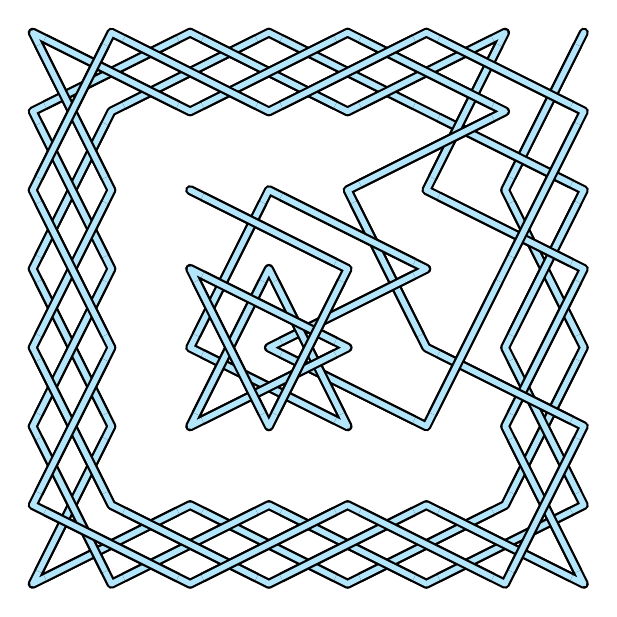
\begin{tikzpicture}[line join=round, line cap=round]
    \draw[overdouble=cyan!30] 
        (7.5,7.5)--(6.5,5.5)--(7.5,3.5)--(6.5,1.5)--(4.5,0.5)--(2.5,1.5)--(0.5,0.5)--(1.5,2.5)--(0.5,4.5)--(1.5,6.5)--(3.5,7.5)--(5.5,6.5)--(7.5,5.5)--(6.5,3.5)--(7.5,1.5)--(5.5,0.5)--(3.5,1.5)--(1.5,0.5)--(0.5,2.5)--(1.5,4.5)--(0.5,6.5)--(2.5,7.5)--(4.5,6.5)--(6.5,7.5)--(5.5,5.5)--(7.5,4.5)--(6.5,2.5)--(7.5,0.5)--(5.5,1.5)--(3.5,0.5)--(1.5,1.5)--(0.5,3.5)--(1.5,5.5)--(0.5,7.5)--(2.5,6.5)--(4.5,7.5)--(6.5,6.5)--(4.5,5.5)--(5.5,3.5)--(7.5,2.5)--(6.5,0.5)--(4.5,1.5)--(2.5,0.5)--(0.5,1.5)--(1.5,3.5)--(0.5,5.5)--(1.5,7.5)--(3.5,6.5)--(5.5,7.5)--(7.5,6.5)--(6.5,4.5)--(5.5,2.5)--(3.5,3.5)--(5.5,4.5)--(3.5,5.5)--(2.5,3.5)--(4.5,2.5)--(3.5,4.5)--(2.5,2.5)--(4.5,3.5)--(2.5,4.5)--(3.5,2.5)--(4.5,4.5)--(2.5,5.5)
    ;
\end{tikzpicture}
\end{document}
